\section{计算机视觉现状}
%做什么,怎么做,比较分析

随着深度神经网络的蓬勃发展,研究人员将其引入计算机视觉各子任务,如图像识别、目标检测、语义分割、人体姿态检测等,均取得了远超以往水平的成果。本章节从图像识别、目标检测、语义分割、实例分割、人体姿态检测这5个方面介绍现有技术的发展。

\subsection{图像识别}
图像识别任务需要将图片归类到给定种类中某一个。自2012年AlexNet在多个视觉竞赛中夺冠,深度神经网络就开始统治图像识别领域。此后,图像识别的研究集中于改进深度神经网络结构,涌现出GoogLeNet、VGG、ResNet等网络,在网络深度、卷积核、浅层信息利用等方面取得了很多成果,将图像识别推向实用化。同时,图像识别也是其他计算机视觉任务的基础,优秀的图像识别网络常被当作其他视觉任务的基础网络;GoogLeNet、ResNet的设计思路被广泛用于其他网络设计中。

\subsection{目标检测}
目标检测(object detection)任务需要识别图片中不同物体的种类,并且用矩形框标出物体的位置,如图\ref{fig:目标检测}。卷积神经网络在图像识别上取得巨大突破后,研究人员开始将其应用在目标检测中。现有的目标检测算法可以分为one-stage和two-stage两类。
\begin{figure}
    \centering
    \subfigure[]{
        \begin{minipage}[t]{0.45\linewidth}
        \centering
        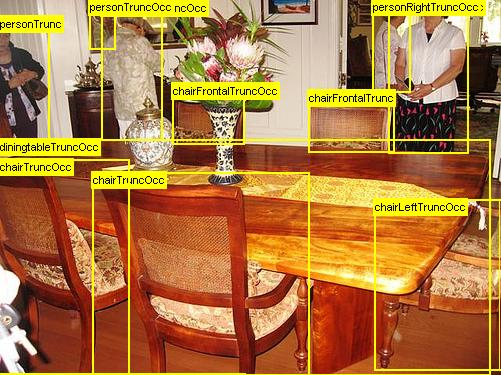
\includegraphics[width=0.8\linewidth]{AI/figures/目标检测-1.jpg}
        \end{minipage}
    }
    \subfigure[]{
        \begin{minipage}[t]{0.45\linewidth}
        \centering
        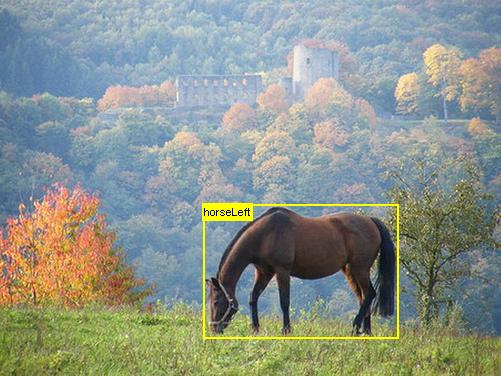
\includegraphics[width=0.8\linewidth]{AI/figures/目标检测-2.jpg}
        \end{minipage}
    }
    \caption{目标检测}
    \label{fig:目标检测}
\end{figure}

\subsubsection{two-stage算法}
two-stage算法将目标检测分为两步:产生候选区域和对候选区域分类。这种思路较为直观,对应算法只需要在图像识别的基础上增加了产生候选区域模块即可。
\textbf{R-CNN}\cite{girshick2014rich}算法是深度神经网络在目标检测领域最早的实践,其主要过程分为四步:首先利用Selective Search算法在图像中生成1000-2000个候选区域;然后将其归一化为统一尺寸后送入卷积神经网络提取特征;神经网路输出的特征送入每一类对应的SVM二分类器分类;最后使用回归器精细修正候选框位置。R-CNN的每个候选框都需要归一化后送到神经网路提取特征,计算量大。

\textbf{SPP-net}\cite{he2015spatial}简化了R-CNN的第二步。先将单张图片送入神经网路提取特征,得到一张特征图,随后对每个候选框区域空间金字塔池化(Spatial Pyramid Pooling,SPP),得到多个固定大小的特征向量。算法核心是空间金字塔池化,它利用特殊的池化层将不同大小的特征图转化为相同大小的特征向量,效果优于暴力拉伸缩放。
\textbf{Fast R-CNN}\cite{girshick2015fast}借鉴SPP-net,做了两点改进:1.简化空间金字塔池化为ROI(Region of interest) pooling。ROI是表示预选框位置的五维矩阵,包括图片索引和左上角右下角坐标。pooling过程如图\ref{fig:ROI},根据ROIs和前层得到的特征图,将候选框分割为预设尺寸的小块;寻找每个小块的最大值;最终得到输出矩阵。2.利用神经网络取代原先的类别分类和位置回归。为此需要多任务损失函数。
\begin{figure}
    \centering
    \subfigure[]{
        \begin{minipage}[t]{0.25\linewidth}
        \centering
        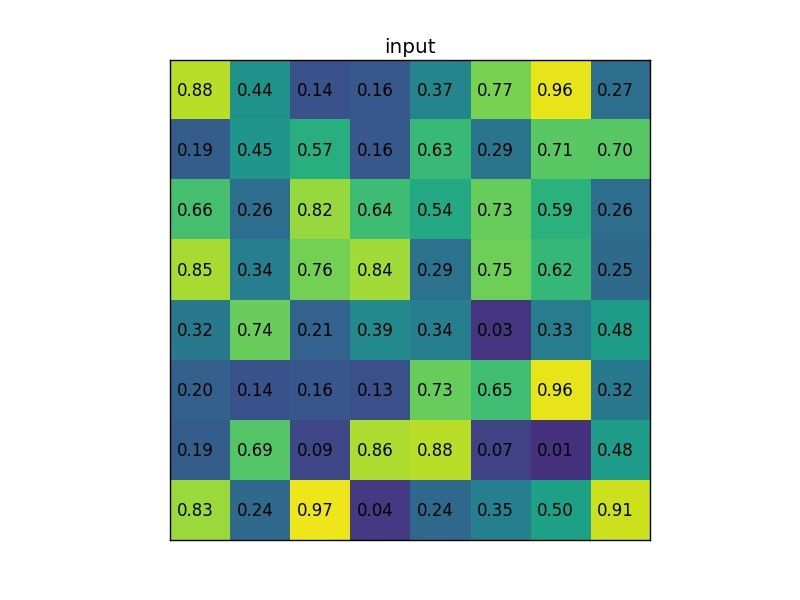
\includegraphics[width=1in]{AI/figures/ROI-1.jpg}
        \end{minipage}
    }
    \subfigure[]{
        \begin{minipage}[t]{0.25\linewidth}
        \centering
        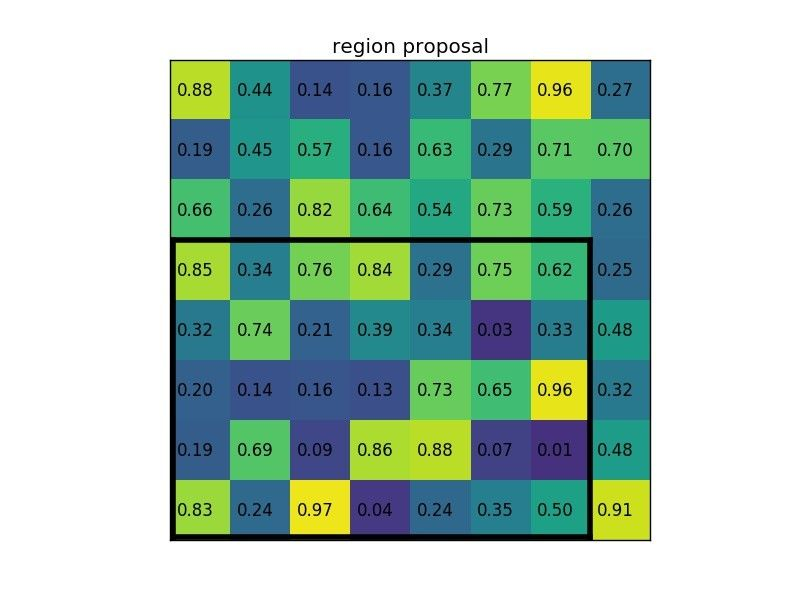
\includegraphics[width=1in]{AI/figures/ROI-2.jpg}
        \end{minipage}
    }
    \subfigure[]{
        \begin{minipage}[t]{0.25\linewidth}
        \centering
        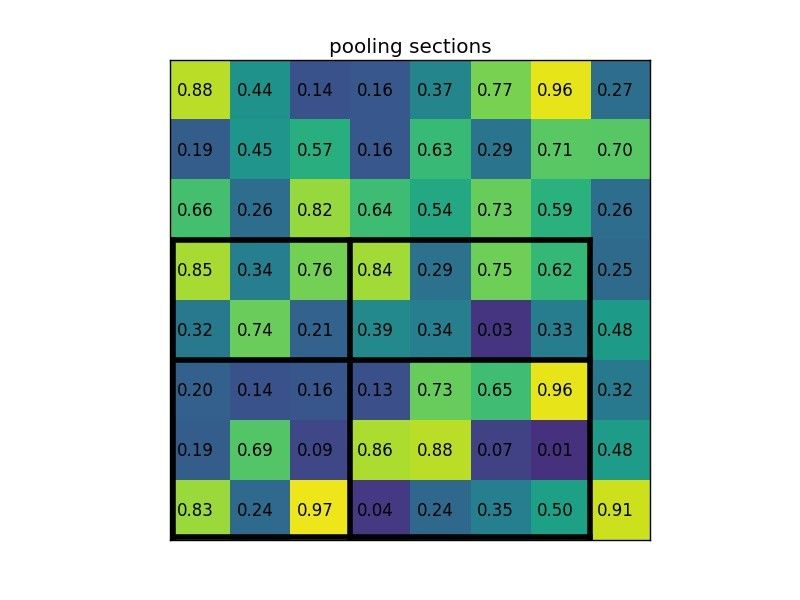
\includegraphics[width=1in]{AI/figures/ROI-3.jpg}
        \end{minipage}
    }
    \subfigure[]{
        \begin{minipage}[t]{0.25\linewidth}
        \centering
        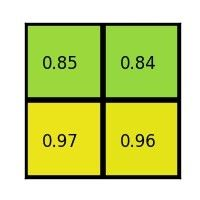
\includegraphics[width=1in]{AI/figures/ROI-4.jpg}
        \end{minipage}
    }
    \caption{ROI pooling}
    \label{fig:ROI}
\end{figure}

从R-CNN升级到Fast R-CNN,整个算法还剩下一个瓶颈:生成候选框。\textbf{Faster R-CNN}\cite{ren2015faster}放弃了传统候选框生成算法Selective Search,设计了RPN(Region Proposal Network)。RPN的输入与ROI pooling的输入相同,而且这两层均为单层卷积层,整个算法变成全卷积结构。故对于单张图片,只需要运行一次神经网络,节省大量计算开销。RPN生成候选框的过程如下:对于特征图的每个点,生成k个anchor boxes(一般设置3种scale和3种aspect rations,共9个anchor boxes)。每个anchor box预测6个参数,2个为存在物体和不存在物体的概率,另外4个是坐标。如果送入RPN的特征图尺寸为W*H,则预测W*H*k个anchor boxes,可以通过nms等方法过滤。

\subsubsection{one-stage算法}
one-stage的解决思路是利用单个卷积神经网络,直接输出预测框的位置信息和物体类别,代表者是YOLO\cite{redmon2016you,redmon2017yolo9000}和SSD\cite{liu2016ssd}。\textbf{YOLO}将预测框和分类两个任务合并,利用利用卷积层提取信息,全连接层输出类别与位置。检测过程先将输入的图片划分为S*S个cell,每个cell负责预测中心点落在该cell的物体的类别和位置。一个cell预测B个bounding box,B个bbox共享类别概率,输出一组5*B+class\_num维结果。以B=2,class\_num=5为例,每个cell输出为:
$$
[x_1,y_1,w_1,h_1,c_1,x_2,y_2,w_2,h_2,c_2, class_1 .... class_5]
$$
YOLO另一个创新是损失函数。传统的目标检测算法中,类别是分类问题,定位是回归问题;而YOLO将两者统一为回归问题,最近预测每个类别的概率而不是二分类。

\textbf{SSD}与YOLO都采用单个神经网络实现分类定位,如图\ref{fig:SSDvsYOLO}。相对于YOLO,SSD作了以下改进:借鉴ResNet的思路,将浅层的特征图连接到最后一层,显著提高了模型的准确度,特别是对小目标的识别能力;以Faster R-CNN的Anchor Box代替YOLO的Bounding Box;网络中部分使用DeepLab提出的空洞卷积。
\begin{figure}
    \centering
    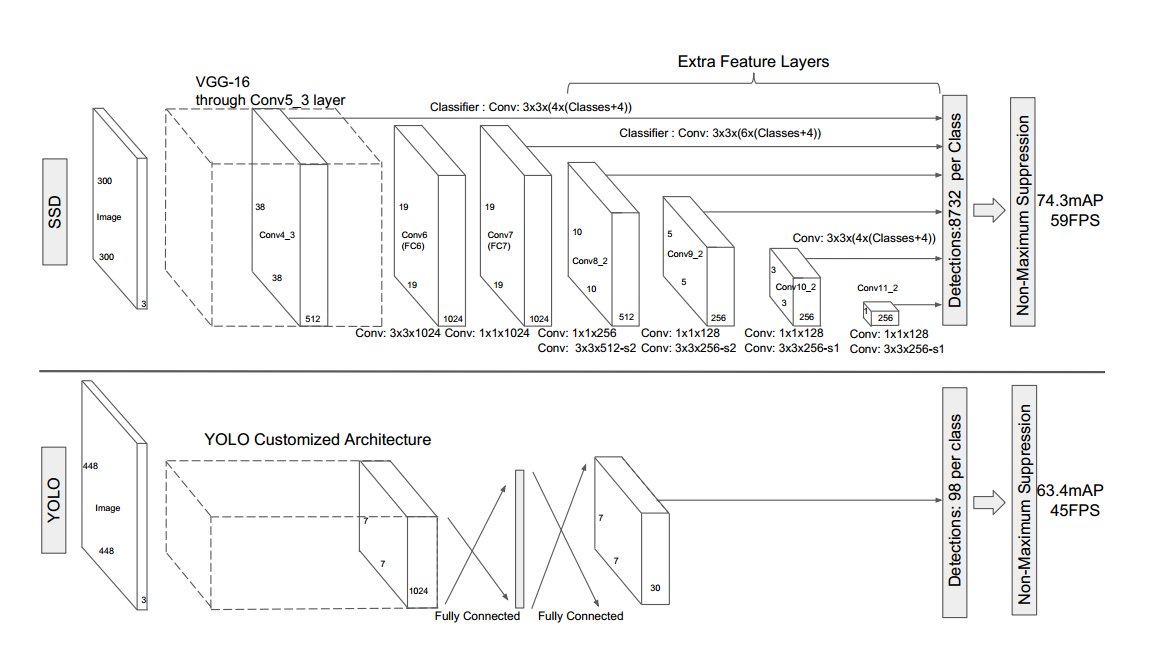
\includegraphics[width=0.7\linewidth]{AI/figures/SSDvsYOLO.png}
    \caption{SSD与YOLO}
    \label{fig:SSDvsYOLO}
\end{figure}

早期one-stage算法和two-stage算法有明显的差异,Fast R-CNN精度高速度慢,YOLO/SSD精度低速度快。但是随着研究的深入,两者的差异越来越小,改进思路趋同。Faster R-CNN可以通过减少预选框的数量,降低精度提高速度;SSD 可以增加网格数量提高精度降低速度\cite{huang2017speed}。R-CNN算法最近的改进,如Grid R-CNN\cite{lu2018grid},融入了网格思想,提高了预测精度。

\subsection{语义分割}
语义分割(Semantic Segmentation)任务需要对输入图片像素级别的分割。可以认为这是更进一步的目标检测,不再用矩形框表示位置,而是用像素点的分类。

\textbf{FCN}\cite{long2015fully}是深度学习在语义分割上的开山之作,借鉴很多现有深度神经网络结构,如图\ref{fig:FCN}。在VGG、GoogLeNet等深度神经网络中,输入图片经过大量卷积层和池化层后,得到的特征图尺寸远小于原尺度。而对于语义分割任务,小尺寸特征图不足以进行像素级别的分割。为了解决这个问题,FCN提出了上采样层结构,即将下采样层(卷积层和池化层)得到的特征图,送入上采样层(反卷积层)恢复到原有的尺寸。由于下采样层一直在减小输出的尺寸,其最后一层输出的特征图信息丢失严重,FCN将多个尺寸的特征图叠加以提高预测精度,即跳层连接(skip connections)。以FCN-16s为例,将con7得到的1*1的特征图上采样为2*2之后和pool4之后的2*2的特征图组合,得到16倍上采样(即与输入相同的尺寸的输出),与原始的FCN相比,预测精度显著提高。FCN将整个网络分为下采样和上采样两部分,此后的语义分割模型大多按照这个思路设计、改进。
\begin{figure}
    \centering
    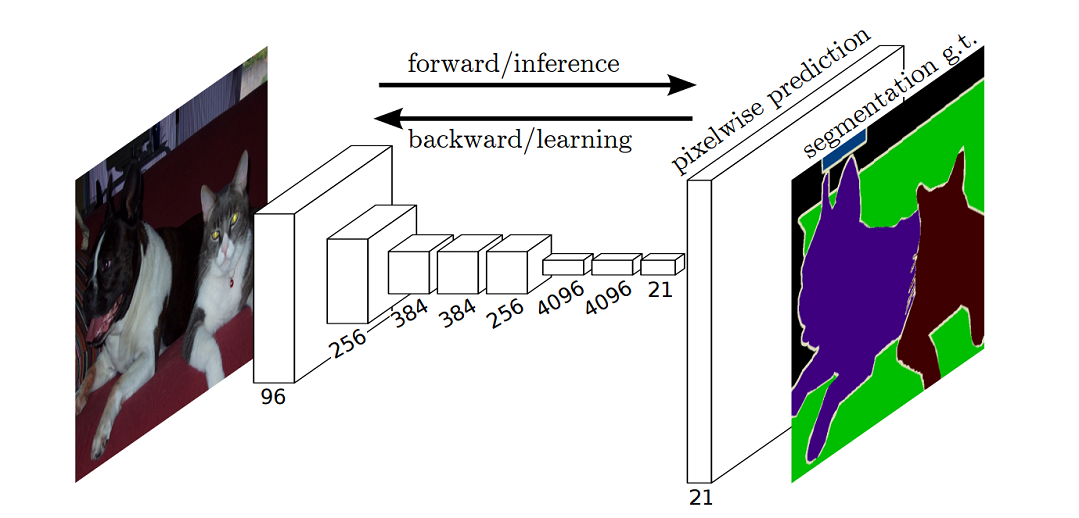
\includegraphics[width=0.7\linewidth]{AI/figures/FCN.png}
    \caption{FCN}
    \label{fig:FCN}
\end{figure}

FCN存在很多问题,它虽然结构对称,但是从参数角度,其下采样层参数占网络总参数的90\%以上。\textbf{SegNet}借鉴FCN的思路:先下采样,后上采样,并将上采样部分称为编码,下采样称为解码。但是与FCN采用skip connections融合浅层信息不同,SegNet将不同卷积层的输出连接到反卷积层的不同位置,如图,这也有利于减小上采样和下采样的参数差距。此外,SegNet还改进了池化层,编码部分的池化层结果保存对应坐标,用于解码还原,保留信息,提高准确率。如图,池化后的6对应一个坐标(1,1),8对应(1,3),在对应的decoder层,将池化结果n*n还原为2n*2n,每个数字还原到对应的位置,其他位置置0(靠反卷积层学习这些位置的数值)。

之前的语义分割,比如FCN,主要依靠池化层进行下采样,降低图像的像素并且增大感知野,之后利用反卷积上采样将图像恢复到原来的尺寸,并且将卷积过程中的不同尺寸的特征图结合提高性能;SegNet将网络分为编码和解码(encoder and decoder)两部分,将编码后得到的特征图与指定解码部分连接,并记录编码部分池化层位置以提高信息利用率。这些算法都遵循一个思路:利用池化减小图像尺寸以增大感受野,随后上采样还原图像尺寸。

利用池化层增大感知野会造成图像尺寸减小、导致信息丢失,而上采样不能完全恢复这些信息。\textbf{DeepLab、Dilated Convolutions}\cite{yu2015multi,chen2018deeplab}等提出了空洞卷积。利用空洞卷积替代池化层,既可以增大感知野,又不会减小图像尺寸。同时,DeepLab引入CRF处理神经网路得到的分割结果,使得最终结果更可靠。现在,DeepLab及其改进是语义分割任务最常见的算法。

\subsection{实例分割}
实例分割(Instance Segmentation)任务是目标检测与语义分割的结合,既需要将物体像素级别分割,又需要识别出分割后物体的类别。它与语义分割的不同之处在于是否区分属于相同类别的不同实例。例如,当图像中存在多只猫,语义分割认为所有猫所在所有像素点均属于猫;而实例分割需要区分出不同像素点分属与不同的猫。

实例分割算法往往是目标检测和语义分割现有算法的集成。\textbf{SDS}\cite{de2017semantic}在AlexNet的基础上增加了SVM,nms等方法,首次使用深度神经网络解决实例分割任务。最新研究将Faster R-CNN与FCN结合,得到\textbf{Mask R-CNN}\cite{he2017mask},效果显著提高,并且可以单独输出目标检测或者语义分割的结果。

\subsection{人体姿态检测}
人体关键点检测(Human\,Keypoint\,Detection)任务需要定位人体的关键点(一般为关节,面部五官)以表示人体姿态,也称为人体姿态估计、人体姿态检测(如图\ref{fig:keypoint}),在行为识别、人机交互、游戏、动画等领域有着很广阔的应用前景。姿态检测算法分为两大类,单人姿态估计和多人姿态估计。

也有将姿态检测分为基于检测(detection-based)的方法和基于回归(regression-based)的方法:基于检测的方法是基于热度图的,对每个关节都生成所有位置的似然热度图,选择概率最大的位置作为该关节的位置。这种方法的缺点是:1. 取概率最大值的操作是不可微分的,所以无法使用端到端的训练方法;2. 由于深度神经网络的降采样操作,热度图的分辨率远低于输入图片的分辨率,这将导致不可逆的量化误差,关节位置的精度会因此受到限制。而使用更高分辨率的热度图,会产生更多的内存和计算开销。

多人姿态估计姿态检测一般有两种方法,一种是自顶向下(Top-down),即先检测图片中人体位置,再检测出该人体的关键点,得到姿态,准确度较高但是速度慢;一种是自底向上(Bottom-up),即先检测出图片中的关键点,再分配给图中的人体,速度快但是准确性较低。



\begin{figure}
    \centering
    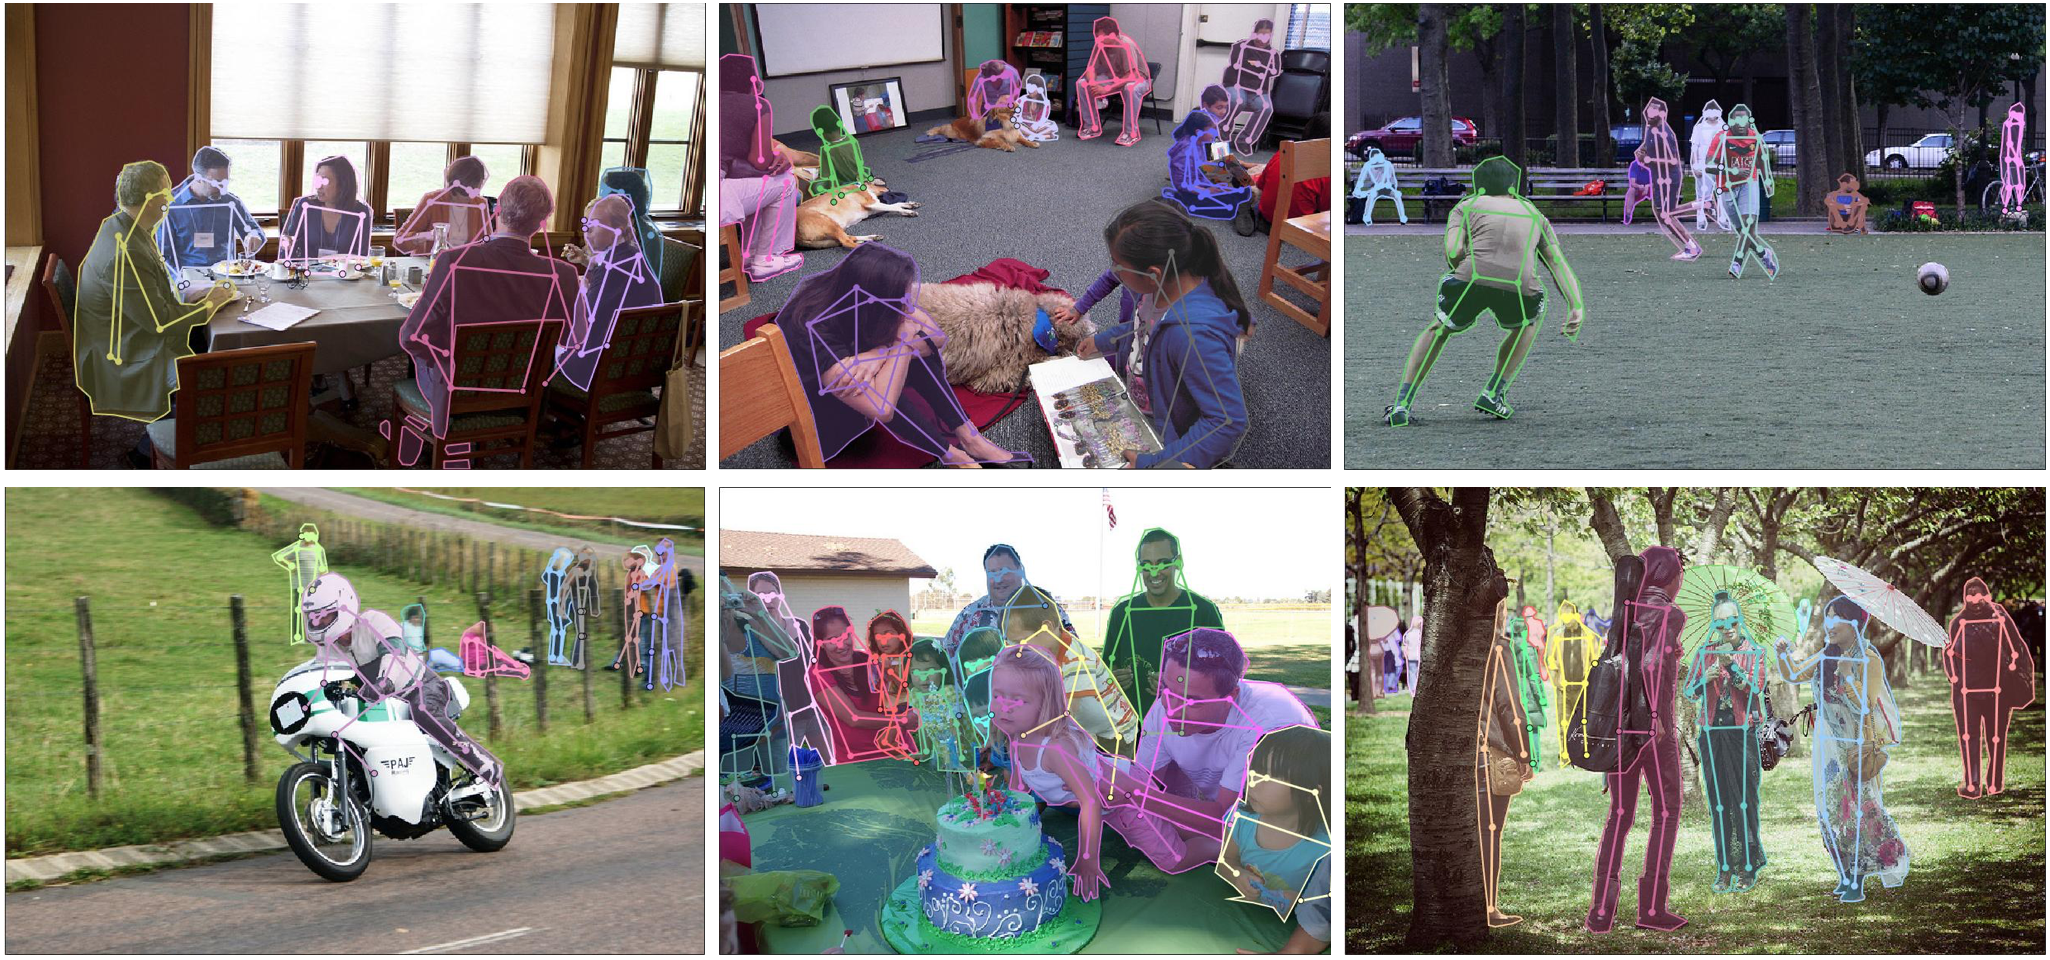
\includegraphics[width=0.7\linewidth]{AI/figures/keypoints-splash-big.png}
    \caption{人体姿态检测}
    \label{fig:keypoint}
\end{figure}

